\section{Parametrization of the orbital configuration}
\label{sec:parameterization}

The current work applies a Walker-Star-type constellation \cite{walker1971, wertz2001ocdm} as the orbital configuration setup. 
It is parameterized by the set of parameters $h, i, S, P, \Delta\Omega, f$, where $h$ is the altitude 
of every circular orbit in the constellation, $i$ is the corresponding orbital inclination, 
$S$ is the number of satellites per orbital plane, $P$ is the number of orbital planes, $\Delta\Omega$ 
is the difference in the right ascension of the ascending node (RAAN) between adjacent planes, 
and $f$ is the interplanar phase shift in the argument of latitude (AOL), which, unlike in the 
traditional Walker description, is specified directly as an angular quantity. In addition, 
$\alpha$ denotes the half-angle of the satellite field-of-view cone measured from the 
subsatellite direction.

The analytical geometric conditions for continuous coverage proposed further in this work assume 
the Earth to be a sphere of radius $R_E$, the equatorial radius of Earth. Therefore, due to the 
symmetry of the Walker Star configuration with respect to rotation about the Earth axis, without loss 
of generality, the RAAN of the first orbital plane is not parameterized and is set equal to $0^\circ$ 
throughout the paper. Furthermore, in the implemented parameterization, unlike in the classical one, 
no requirement is imposed for the RAAN of the last plane to be equal to $180^\circ$.

Based on these parameters, several key geometric relations are introduced below 
and are subsequently applied in further coverage assessments.

\subsection{Sattelite coverage geometry}
A Walker Star constellation assumes that all satellites are located in circular orbits 
at altitude $h$. Each satellite covers a certain spherical cap on the surface of Earth, 
whose size is determined by the corresponding central angle $\theta$. The angle $\theta$ is 
constrained by the field-of-view half-angle $\alpha$, which is determined by the satellite payload 
characteristics. The relation between these angles follows directly from the geometrical conditions:

\begin{equation}
    \frac{R_E}{\sin\alpha}=\frac{\left|\mathbf{R}_{\mathrm{sat}}\right|}{\sin(\alpha+\theta)}.
\end{equation}

In an ideal case, $\left|\mathbf{R}_{\mathrm{sat}}\right|=R_E+h$, and therefore the central angle 
of the covered spherical cap can be expressed as:

\begin{equation}
        \theta=\arcsin\left[\left(1+\frac{h}{R_E}\right)\sin\alpha\right]-\alpha.
\end{equation}

\begin{figure}[ht]
    \centering
    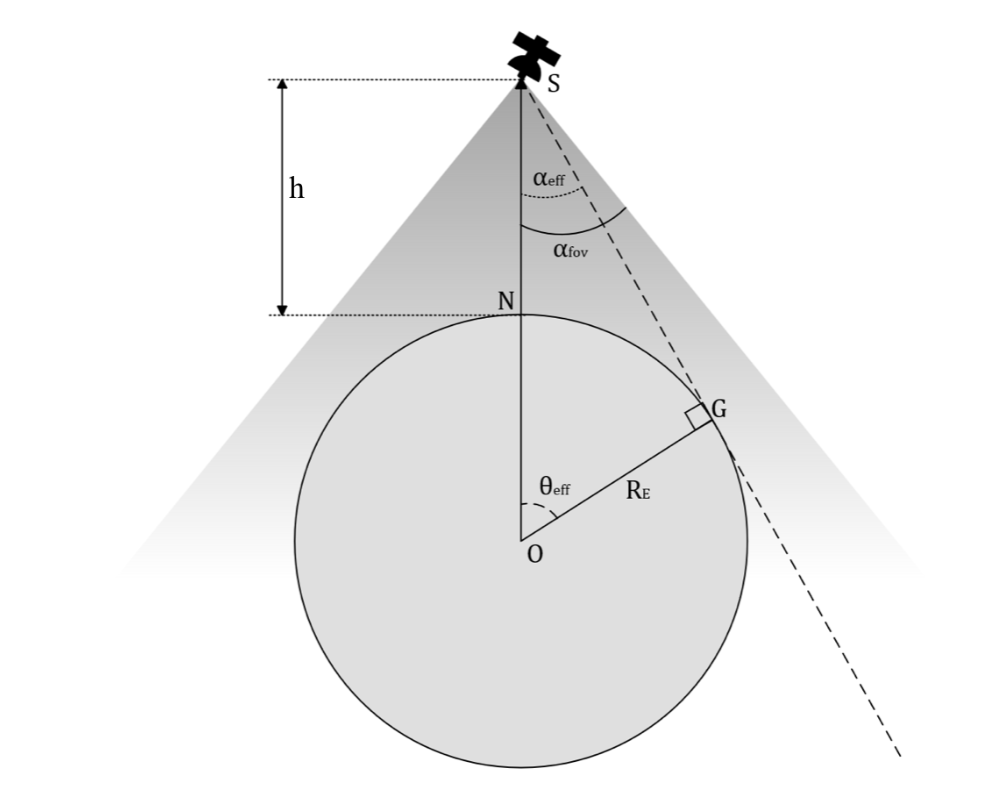
\includegraphics[width=0.75\textwidth]{pictures/effective_fov.png}
    \caption{Single sattelite effective field-of-view}
    \label{fig:effective_fov}
\end{figure}

In cases where the field-of-view half-angle $\alpha$ extends beyond the Earth limb, an additional 
constraint is required. The effective field-of-view half-angle $\alpha_{\mathrm{eff}}$ is therefore 
introduced as the maximum angle at which the surface of Earth can be observed from a given altitude. 
From the simple geometrical relation (Fig.~~\ref{fig:effective_fov}), this limiting angle is given by

\begin{equation}
        \alpha_{\mathrm{eff}}=\arcsin\left[\frac{R_E}{\mathbf{R}_{\mathrm{sat}}}\right]=\arcsin\left[\frac{R_E}{R_E+h}\right].
\end{equation}

Thus, the field-of-view half-angle used in the further calculations can be defined as:

\begin{equation}
\alpha^{*} = \min\left(\alpha,\alpha_{\mathrm{eff}}\right)
\end{equation}

\subsection{Street-of-coverage}

\begin{figure}[ht]
    \centering
    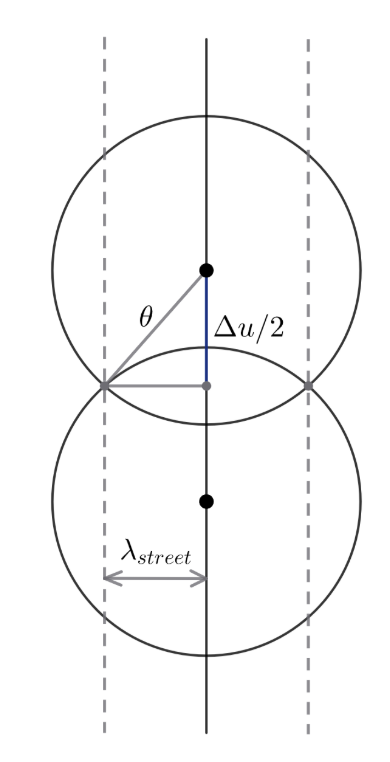
\includegraphics[width=0.5\textwidth]{pictures/lambda_street.png}
    \caption{Single orbital plane street-of-coverage}
    \label{fig:lambda_street}
\end{figure}

In order for several satellites within a single orbital plane to provide continuous coverage, 
it is not sufficient for their instantaneous coverage regions to simply touch. The coverage regions 
of neighboring satellites must overlap, forming a continuous street-of-coverage along the ground track \cite{ulybyshev2014, wertz2001ocdm}. 
The angular half-width of this street, denoted by $\lambda_{\mathrm{street}}$, can be obtained by applying 
the spherical law of cosines to the spherical triangle shown in Fig.~~\ref{fig:lambda_street}:

\begin{equation}
\lambda_{\mathrm{street}} = \arccos\left(\frac{\cos\theta}{\cos\left(\Delta u/2\right)}\right)
\end{equation}

where $\Delta u$ is the AOL between neighboring satellites within the same orbital plane. 

\subsection{Angular separation between orbital planes}

To ensure global coverage, this paper considers conditions on the maximum allowable angular 
distances between orbital planes. The angular distance between circular orbits, denoted 
as $i_{\mathrm{rel}}$, is defined as the largest angular distance between the corresponding orbits.
The angle between two orbital planes is equal to the angle between their normal vectors. 
For an orbital plane, based on the definitions of RAAN $\Omega$ and inclination $i$, the normal vector 
is expressed as follows:

\begin{equation}
\mathbf{n}=
\left(
\sin\Omega\sin i,
-\cos\Omega\sin i,
\cos i
\right),
\end{equation}

where the direction of the normal vector is determined by the direction of the orbital 
angular momentum vector $\mathbf{r}\times\mathbf{v}$.
Based on the equality of inclinations of the Walker constellation orbital planes, 
for any two orbital planes the angular distance between them is calculated as

\begin{equation}
\cos i_{\mathrm{rel}}=\frac{\mathbf{n}_1\cdot\mathbf{n}_2}{|\mathbf{n}_1||\mathbf{n}_2|}=\cos^2 i+\cos(\Omega_2-\Omega_1)\sin^2 i.
\end{equation}

For neighboring orbital planes, this angular distance is

\begin{equation}
i_{\mathrm{rel}}=\arccos\left(\cos^2 i+\cos\Delta\Omega,\sin^2 i\right).
\end{equation}

For the angular distance between the first and the last orbital planes, the RAAN difference is $(P-1)\Delta\Omega$, and therefore

\begin{equation}
i_{\mathrm{rel}}=\arccos\left(\cos^2 i+\cos\left((P-1)\Delta\Omega\right)\sin^2 i\right).
\end{equation}

For the supplementary angular distance, which will be used further for the retrograde case,
\begin{equation}
i_{\mathrm{rel}}=\pi-\arccos\left(\cos^2 i+\cos\left((P-1)\Delta\Omega\right)\sin^2 i\right).
\end{equation}
